\documentclass[12pt]{article}

% please note that this paper uses the ams symbols so that the
% amssymb.sty is included.  If you don't use these then you can
% exclude the next line.  This paper requires the ams symbols to compile.
%  You might also use other standard style files such as amsmath, latexsym, etc
% all of these should be included in the usepackage statement on the next line.

\usepackage{amsmath,amsthm,amssymb,euscript,amscd}
\usepackage[english]{babel} % espanol, 
\usepackage[utf8]{inputenc} % acentos sin codigo
\usepackage{graphicx}
\usepackage{url}
\usepackage{hyperref}
\usepackage{bm}
\usepackage{rotating}
\usepackage{fancyhdr}
\pagestyle{fancy}
\fancyhf{} 

\fancyfoot[R]{\thepage}
% the most common useage to include a graphic scaled by .5
%(on a scale of 0 to whatever with 1 the actual size.)
%
% \centerline{  \includegraphics[scale=.5]{filename.eps}  }
%
%  there are of course many variation on this theme.


\lhead{
\includegraphics[width=.24\textwidth]{imagenes/logo.png}}
\renewcommand{\headrulewidth}{0pt}
\renewcommand{\footrulewidth}{0pt}
\setlength\headheight{30.0pt}
\addtolength{\textheight}{00.0pt}

 %----------------------

%%%%%  page size setting for United States %%%%%%%%%%%%%

\setlength{\textwidth}{6.5in}
\setlength{\textheight}{8.0in} %
%\setlength{\hoffset}{-.5in} %
\setlength{\topmargin}{-.5in}
\setlength{\evensidemargin}{0in}
\setlength{\oddsidemargin}{0in}


%%%%%%%%%%%%%%%%%%%%%%%%%%%%%%%%%%%%%%%


\renewcommand{\baselinestretch}{1.1}

\parskip=0pt
\parindent=10pt


\title{Advanced Simulation of Electric \\ Power Distribution Systems}
\author{Paulo M. De Oliveira-De Jesus\thanks{\url{pm.deoliveiradejes@uniandes.edu.co}} \\
Electrical \& Electronic Engineering Dept.\\
 
\includegraphics[width=5cm]{imagenes/logo}}


\begin{document}

\maketitle
\begin{abstract}
This document presents a number of methodologies used to solve the Kersting NEV test system (Power Flow and Short Circuit).
Three network models are considered: positive-sequence (balanced), three-phase (unbalanced), multiphase-multigrounded (4-wire unbalanced).  Solutions allow us to compare voltage profiles, current flow patterns and power losses for different network modelling strategies.
\end{abstract}


\section{Introduction}
\setcounter{equation}{0}

The objective of this document is to illustrate the application of power flow and short-circuit analysis considering different network models:  positive-sequence (balanced), three-phase (unbalanced), multiphase-multigrounded (4-wire unbalanced). To do so, the well-known neutral-to-earth voltage (NEV) test system depicted in Fig \ref{fig:1} is used. This document develops in detail the algorithms required to perform power flow and short circuit studies. 

A number of simple programs were coded in order to take the data from a database, build the network models and perform the power system studies. The idea is to compare the output (voltages, currents and power losses) for different modelling strategies. Solutions obtained are also validated using two general purpose software: commercial tool Digsilent PowerFactory\footnote{\url{https://www.digsilent.de/en/}} and EPRI's open-source platform OpenDSS\footnote{\url{smartgrid.epri.com/SimulationTool.aspx}}.

The main program is depicted in Fig. \ref{fig:2}. This program was coded in Octave. Octave is free and it can be downloaded at \url{https://www.gnu.org/software/octave/}. It comprises four parts: 1) Data input routines;
  2) Modelling routines: source, network and load; 3) Power Flow routines and 4) Short-circuit routines.
The first part includes the function {\em [db]=loaddatabase} that calls all data required to determine the system models and power flow calculations. In this case, system data is related to the NEV system presented by Kersting \cite{1}. The second part includes three functions  {\em generation.m},  {\em network.m} and  {\em demand(db)}. The source model is defined according to the short-circuit level and the X/R ratio at grid supply point (GSP). In this case, the GSP is denoted as node 1. The network function determines the $\pi$ model of the NEV test system for multigrounded, three-phase and positive sequence representations. The load function defines three-phase and positive sequence constant power (active and reactive) at demand side.

The third and fourth part of the code depicted in Fig. \ref{fig:2} perform different types of power flow and short-circuit analyses according to the network model adopted. Next, detailed explanation of each function is provided.

\begin{figure}[hbt]
  \centering{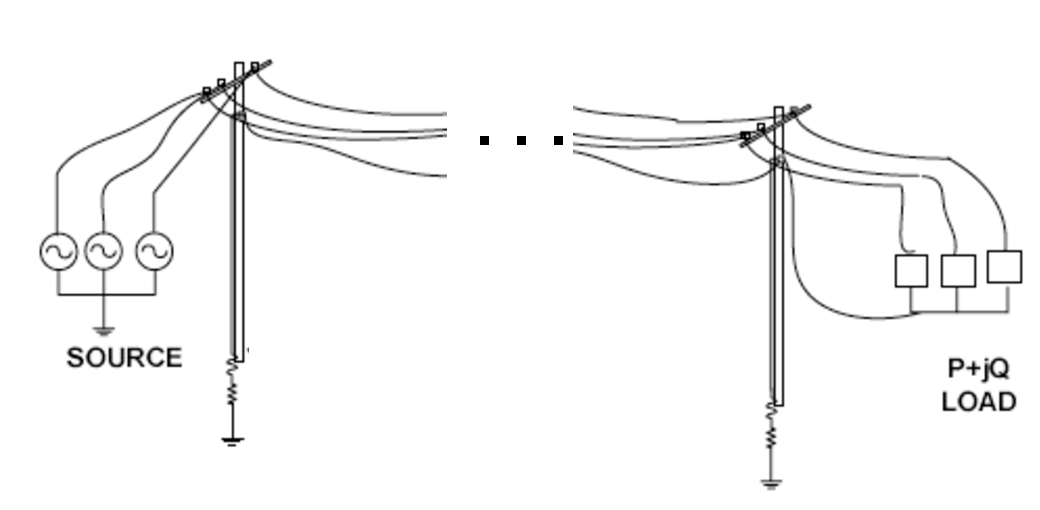
\includegraphics[width=3in]{images/nev.pdf}
  \caption{The NEV test system}\label{fig:1}}
\end{figure}
\begin{figure}[hbt]\centering{
  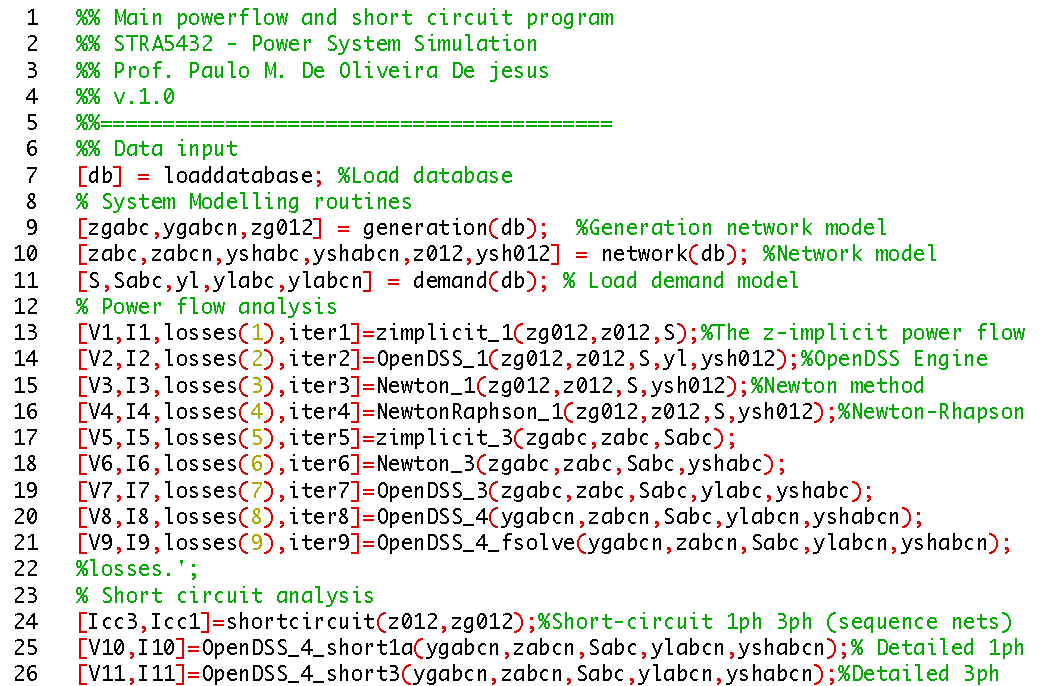
\includegraphics[width=5in]{images/octave.pdf}
  \caption{Main program}\label{fig:2}}
\end{figure}
\newpage



\section{Power system models}

Prior to perform power system analyses such has power flow and  short-circuit, we need to build the system 
model. Three models must be defined: 1) the Th\'evenin equivalent at grid supply point, 2) the network model i.e. the series impedance and shunt admittance elements of the distribution line, and  3) the load model. 

%\begin{figure}[hbt]\centering{
%  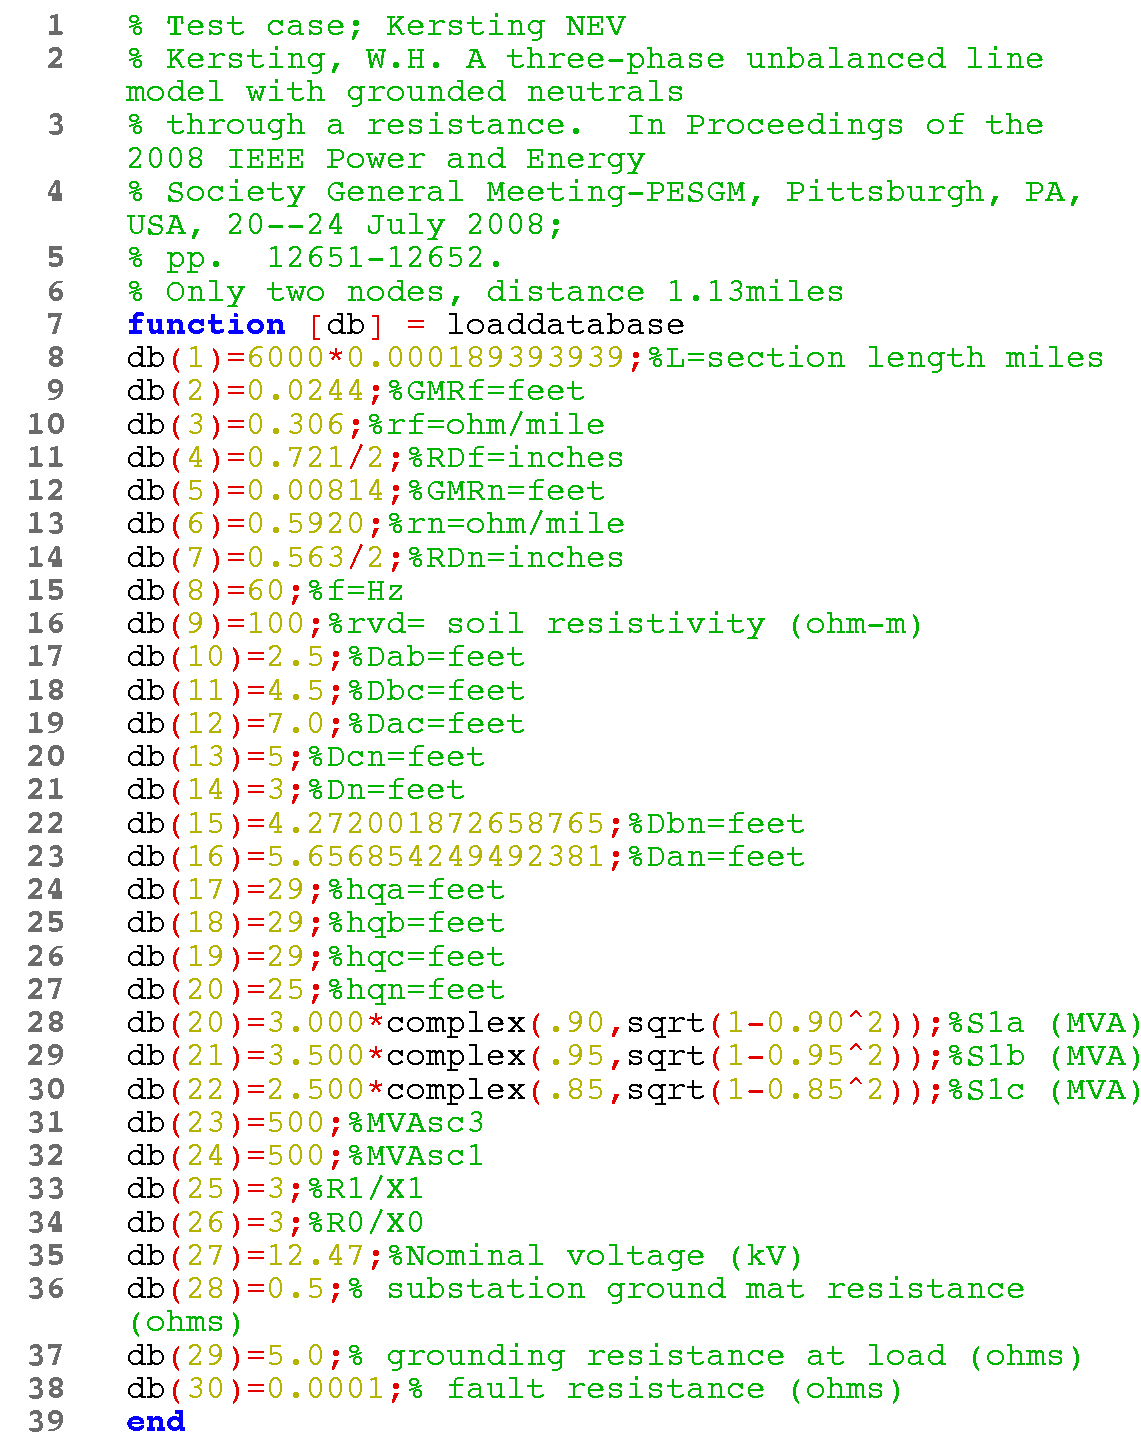
\includegraphics[width=5in]{images/loaddatabase.pdf}
%  \caption{NEV system Database}\label{fig:3}}
%\end{figure}

These models are built according to the {\em loaddatabase(db)} function. The following quantities are determined:
  
\begin{verbatim}
[zg012,zgabc,ygabcn] = generation(db);  %Generation network model 
[z012,zabc,zabcn,ysh012, yshabc,yshabcn] = network(db); %Network model
[S,Sabc,yl,ylabc,ylabcn] = demand(db); % Load demand model 
\end{verbatim}

The \textbf{source model} is defined by the {\em generation(db)} function where

Element \texttt{zg012} is the sequence Th\'evenin equivalent impedance matrix $\mathbf{Z^{0+-}_{G}}$

Element \texttt{zgabc} is the three-phase Th\'evenin equivalent impedance matrix $\mathbf{Z^{abc}_{G}}$ 

Element \texttt{ygabcn} is the 4-wire Th\'evenin equivalent impedance matrix $\mathbf{Y^{abcn}_{G}}$

The \textbf{network model} is defined by the {\em network(db)}  function where

Element \texttt{z012} is the sequence series impedance matrix $\mathbf{Z^{sh,0+-}_{12}}$

Element \texttt{zabc} is the three-phase series impedance matrix $\mathbf{Z^{sh,abc}_{12}}$ 

Element \texttt{zabcn} is the 4-wire series impedance matrix $\mathbf{Z^{sh,abcn}_{12}}$

Element \texttt{ysh012} is the sequence shunt admittance matrix $\mathbf{Y^{sh,0+-}_{12}}$

Element \texttt{yshabc} is the three-phase shunt admittance matrix $\mathbf{Y^{sh,abc}_{12}}$

Element \texttt{yshabcn} is the 4-wire shunt admittance matrix $\mathbf{Y^{sh,abcn}_{12}}$
  
The \textbf{load model} is   defined by the {\em demand(db)}  function where

Element \texttt{S} is the total demand, apparent power ${S}$ 

Element \texttt{Sabc} is the three-phase demand vector $\mathbf{S^{abc}}$ 

Elements \texttt{yl}, \texttt{ylabc} and \texttt{ylabcn} are the load admittances according to Norton equivalents (OpenDSS load model), $\mathbf{Y_{L}}$, $\mathbf{Y^{abc}_{L}}$, $\mathbf{Y^{abcn}_{L}}$ .


\subsection{The Source}

Source Th\'evenin equivalent (sequence parameters): 
Determine positive and zero sequence impedances (${Z}^{+}$, ${Z}^{0}$) when nominal voltage $kVLL$ in kV, short-circuit levels $MVA_{sc1}$ and $MVA_{sc3}$ in MVA, and X1/R1=$\alpha$ X0/R0=$\beta$ relations are specified.
\begin{equation}
Z^{+}=\frac{kVLL^2}{MVA_{sc3}}\mbox{ ohms}
\end{equation}

then,
\begin{equation}
R^{+}=\frac{Z^{+}}{\sqrt{1+\alpha^2}}\mbox{ ohms}
\end{equation}

\begin{equation}
{Z}^{+}={R^{+}}+j{\alpha R^{+}}={R^{+}}+j{X^{+}}\mbox{ ohms}
\end{equation}
\begin{equation}
\gamma=\frac{3 kVLL^2}{MVA_{sc1}}
\end{equation}
then
\begin{equation}
R^{0}=\frac{-b+\sqrt{b^2-4ac}}{2a}\mbox{ ohms}
\end{equation}
where:

$a$=$\beta^2+1$

$b$=$4R_1+4 \beta X_1$

$c$=$4R_1^2+4X_1^2-\gamma^2$

\begin{equation}
{Z}^{0}={R^{0}}+j{\beta R^{0}}={R^{0}}+j{X^{0}}\mbox{ ohms}
\end{equation}

Three phase model: 3x3 source impedance matrix is:

\begin{equation}
\mathbf{Z^{abc}_{G}}=\mathbf{A_S}
\mathbf{Z_{0+-}}
    \mathbf{A_S}^{-1}=\mathbf{A_S}
\left[ \begin{array}{ccc}
               {Z}^{0} & 0 &0\\
               0 & {Z}^{+} & 0  \\
               0 & 0 & {Z}^{+}  \\
             \end{array}
           \right] \mathbf{A_S}^{-1} 
           \mbox{ ohms}
\end{equation}

where

\begin{equation}
\mathbf{A_s}= 
\left[ \begin{array}{ccc}
               1 & 1 &1\\
               1 & a^2 & a  \\
               1 & a & a^2   \\
             \end{array}
           \right]  
           \end{equation}

and $a$=$e^{\frac{j 2  \pi}{3}}$

Three phase model: 3x3 source admittance matrix is:

\begin{equation}
\mathbf{Y^{abc}_{G}}=[\mathbf{Z^{abc}_{G}}]^{-1} \mbox{ siemens}
\end{equation}

Multigrounded model: The 4x4 source admittance matrix is:

\begin{equation}
\mathbf{Y^{abcn}_{G}}=\left[ \begin{array}{cccc}
               {Y}^{aa}_{G}  & {Y}^{ab}_{G}   &{Y}^{ac}_{G}  & -{Y}^{aa}_{G}\\
               {Y}^{ba}_{G} & {Y}^{bb}_{G}  &{Y}^{bc}_{G} & -{Y}^{bb}_{G}\\
               {Y}^{ca}_{G} & {Y}^{cb}_{G}  &{Y}^{cc}_{G} & -{Y}^{cc}_{G}\\
              -{Y}^{aa}_{G} & -{Y}^{bb}_{G} &-{Y}^{cc}_{G} & -{Y}^{aa}_{G}-{Y}^{bb}_{G}-{Y}^{cc}_{G}-\frac{1}{r_1}\\
             \end{array}
           \right] \mbox{ siemens}
           \end{equation}

where $r_1$ is the grounding resistance neutral at source in ohms. 

\subsection{The Network Model}

Series and shunt impedances of a distribution feeder under 4-wire, three-phase and positive sequence models
are determined according to Kersting's book chapters 4 and 5 \cite{2}.
 
\subsection{The Load Model}

Only constant powers (active and reactive are considered). Given a three-phase demand vector $\mathbf{S_{abc}}$=$[{S}_{a},{S}_{b},{S}_{c}]^T$ the total demand is:

\begin{equation}
  {S}={S}^{a}+{S}^{b}+{S}^{c}\mbox{ MVA}
\end{equation}

To perform studies under the OpenDSS philosophy we need to define the following entities:


The positive sequence admittance load is given by a diagonal $n x n$ matrix whose elements are:

\begin{equation}
{Y}^{+}_{L}=\frac{1}{3}\frac{{S}^*}{(V^{nom})^2}\mbox{ siemens} 
\end{equation} 

where $V^{nom}$ is the line-to-line nominal voltage in kV.


Three phase model: 3x3 source impedance matrix is:

\begin{equation}
\mathbf{Y^{abc}_{L}}=diag([{Y}^a_{L},{Y}^b_{L},{Y}^c_{L}]\mbox{ siemens}
\end{equation} 

where ${Y}^p_{L}$=$\frac{1}{3}\frac{({S}^p)^*}{(V^{nom})^2}$, $p$=$a,b,c$.

Multigrounded model: The 4x4 load admittance matrix is:

\begin{equation}
\mathbf{Y^{abcn}_{L}}=\left[ \begin{array}{cccc}
               {Y}^{a}_{L} &0  &0 & -{Y}^{a}_{L}\\
              0 & {Y}^{b}_{L}  &0 & -{Y}^{b}_{L}\\
               0 &0  &{Y}^{c}_{L} & -{Y}^{c}_{L}\\
               -{Y}^{a}_{L} & -{Y}^{b}_{L}  &-{Y}^{c}_{L} & -{Y}^{a}_{L}-{Y}^{b}_{L}-{Y}^{c}_{L}-\frac{1}{r_2}\\
             \end{array}
           \right] \mbox{ siemens}\end{equation}
  
where $r_2$ is the grounding resistance neutral at load in ohms. 

\section{Power Flow Analysis}

\subsection{Power Flow No. 1: Z-implicit (Positive sequence)}

Given the nominal voltage ($v_0=12.47/\sqrt{3}$), the positive sequence source Th\'evenin equivalent impedance (${Z}^{+}_{G}$), the network series impedance (${Z}^{+}_{12}$) and total load (${S}$)
determine voltages ($\bm{v}$), injected currents ($\mathbf{i}$), active power (losses) and computational performance:
    
\begin{verbatim}
  function [V,I,losses,iter]=zimplicit_1(zg012,z012,S)
\end{verbatim}

Shunts admittances are neglected.

\begin{figure}[hbt]\centering{
  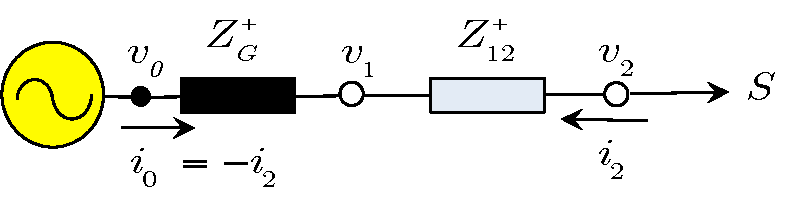
\includegraphics[width=4in]{images/pf1.pdf}
  \caption{Positive sequence power flow}\label{fig:4}}
\end{figure}
\newpage

Starting with ${v}_2$=$v_0$=$12.47/\sqrt{3}$, using KVL we update ${v}^{new}_2$ as

\begin{equation}
  {v}^{new}_2=v_0+({Z}^{+}_{G}+{Z}^{+}_{12})\cdot \frac{-{S}^*}{{v}^*_2}\mbox{ kV}
\end{equation}

where ${Z}^{+}_{G}$=${Z}^{0+-}_{G}(2,2)$ and ${Z}^{+}_{12}$=${Z}^{0+-}_{12}(2,2)$

After a number of iterations (\textit{iter}) when $\mid{v}^{new}_2-{v}^{old}_2\mid\leq \epsilon$ the loop stops. Thus, voltage at bus 1 is:

\begin{equation}
  {v}_1=v_0+{Z}^{+}_{G}\cdot \frac{-{S}^*}{{v}^*_2}\mbox{ kV}
\end{equation}

In matrix notation resulting voltages and currents are:

\begin{equation}
  \bm{v}=[{v}_0, {v}_1,{v}_2]^T
\end{equation}
\begin{equation}
  \bm{i}=[-{i}_2,0,{i}_2]^T
\end{equation}
where ${i}_2$=$(\frac{-{S}}{{v}_2})^*$ and  ${i}_0$=-${i}_2$.

Applying the Tellegen's theorem, power losses at the line are: $\Delta {S}$=$\Delta P$+j$\Delta Q$ 
=$3*[{v}_1,{v}_2][-{i}^*_2,{i}^*_2]^T$

\subsection{Power Flow No. 2: OpenDSS solution (Positive sequence)}

Given the nominal voltage ($v_0=12.47/\sqrt{3}$), the positive sequence source Th\'evenin equivalent impedance (${Z}^{+}_{G}$), the network series impedance and shunt admittance (${Z}^{+}_{12}$, ${Y}^{sh,+}_{12}$), the load equivalent (${Y}^{+}_{L}$) and total load (${S}$)
determine voltages ($\bm{v}$), injected currents ($\mathbf{i}$), active power (losses) and computational performance:
    
\begin{verbatim}
[V,I,losses,iter]=OpenDSS_1(zg012,z012,S,yl,ysh012);%OpenDSS Engine
\end{verbatim}

We need to construct the OpenDSS's admittance matrix as follows

\begin{equation}
\mathbf{Y^{+}_{OpenDSS}}=\left[ \begin{array}{cc}
               {Y}^{+}_{G}+{Y}^{+}_{12}+\frac{
1}{2}{Y}^{sh,+}_{12} &-{Y}^{+}_{12} \\
              -{Y}^{+}_{12}  & {Y}^{+}_{L}+{Y}^{+}_{12}+\frac{
1}{2}{Y}^{sh,+}_{12}
             \end{array}
           \right] \mbox{ siemens}\end{equation}

where  ${Y}^{+}_{G}$= $(Z^{+}_{G})^{-1}$ and
${Y}^{+}_{12}$= $(Z^{+}_{12})^{-1}$.

Starting with ${v}_2$=$v_0$=$12.47/\sqrt{3}$, using KVL we update the compensated injected currents as ${i}_{c1}$ and ${i}_{c2}$ as

\begin{eqnarray}
  {i}_{c1}&=&{Y}^{+}_{G}v_0-\frac{1}{2}{Y}^{sh,+}_{12}v_1\mbox{ kA}\\
    {i}_{c2}&=&{i}_{2}-\frac{1}{2}{Y}^{sh,+}_{12}v_2\mbox{ kA}
\end{eqnarray}

where:   ${i}_2$=$\frac{-{S}^*}{{v}^*_2}$.
 
The updated voltages are:

\begin{equation}
\begin{bmatrix}
	{v}^{new}_1\\ 
	{v}^{new}_2
\end{bmatrix}=
  \mathbf{{Y}^{+}_{OpenDSS}}
  \begin{bmatrix}
  {i}_{c1}\\
  {i}_{c2}\end{bmatrix}
    \mbox{ kV}
\end{equation}

Putting all together the updated voltages are:

\begin{equation}
\begin{bmatrix}
	{v}^{new}_1\\ 
	{v}^{new}_2
\end{bmatrix}=
 \left[ \begin{array}{cc}
               {Y}^{+}_{G}+{Y}^{+}_{12}+\frac{
1}{2}{Y}^{sh,+}_{12} &-{Y}^{+}_{12} \\
              -{Y}^{+}_{12}  & {Y}^{+}_{L}+{Y}^{+}_{12}+\frac{
1}{2}{Y}^{sh,+}_{12}
             \end{array}
           \right]
  \begin{bmatrix}
  {Y}^{+}_{G}v_0-\frac{1}{2}{Y}^{sh,+}_{12}v_1\\
  \frac{-{S}^*}{{v}^*_2}-\frac{1}{2}{Y}^{sh,+}_{12}v_2\end{bmatrix}
    \mbox{ kA}
\end{equation}

After a number of iterations (\textit{iter}) when  $\mid{v}^{new}_1-{v}^{old}_1\mid\leq \epsilon$ and $\mid{v}^{new}_2-{v}^{old}_2\mid\leq \epsilon$ the loop stops. 

Applying the Tellegen's theorem, power losses at the line are: $\Delta {S}$=$\Delta P$+j$\Delta Q$=$3*[{v}_1,{v}_2][-{i}^*_2,{i}^*_2]^T$

\subsection{Power Flow No. 3: Newton Method (Positive sequence)}

Given the nominal voltage ($v_0=12.47/\sqrt{3}$), the positive sequence source Th\'evenin equivalent impedance (${Z}^{+}_{G}$), the network series impedance and shunt admittance (${Z}^{+}_{12}$, ${Y}^{sh,+}_{12}$)and total load (${S}$)
determine voltages ($\bm{v}$), injected currents ($\mathbf{i}$), active power (losses) and computational performance:
    
\begin{verbatim}
[V,I,losses]=Newton_1(zg012,z012,S,ysh012);%Newton method
\end{verbatim}

The idea is find $\bm{v}$=$[{v}_1,{v}_2]^T$ from $\bm{i}$=$\mathbf{Y_{BUS}}\bm{v}$ (Eq. \ref{1}) using an appropriate solver (Octave's {fsolve} tool).


\begin{equation}
 \left[ \begin{array}{ccc}\label{1}
 {Y}^{+}_{G} & - {Y}^{+}_{G}  &0 \\
 - {Y}^{+}_{G} &  {Y}^{+}_{G}+{Y}^{+}_{12}+\frac{1}{2}{Y}^{sh,+}_{12} & -{Y}^{+}_{12}\\
 0 & -{Y}^{+}_{12} & {Y}^{+}_{12}+\frac{1}{2}{Y}^{sh,+}_{12}
             \end{array}
           \right]
  \begin{bmatrix}
  {v}_0\\ 
	{v}_1\\ 
	{v}_2
\end{bmatrix}
  =
     \begin{bmatrix} 
   \frac{{S}^*}{{v}^*_2} \\ 
  0\\ 
  \frac{-{S}^*}{{v}^*_2}
  \end{bmatrix}=
  \begin{bmatrix}
{i}_0=-{i}_2\\ 
0\\ 
{i}_2
\end{bmatrix}
  \end{equation}


Applying the Tellegen's theorem, power losses of the line are: $\Delta {S}$=$\Delta P$+j$\Delta Q$ 
=$3*[{v}_1,{v}_2][-{i}^*_2,{i}^*_2]^T$

\subsection{Power Flow No. 4: Newton-Rapshon Method (Positive sequence)}

Given the nominal voltage ($v_0=12.47/\sqrt{3}$), the positive sequence source Th\'evenin equivalent impedance (${Z}^{+}_{G}$), the network series impedance and shunt admittance (${Z}^{+}_{12}$, ${Y}^{sh,+}_{12}$)and total load (${S}$)
determine voltages ($\bm{v}$), injected currents ($\mathbf{i}$), active power (losses) and computational performance:
    
\begin{verbatim}
[V,I,losses]=NewtonRaphson_1(zg012,z012,S,ysh012);%Newton-Rhapson method
\end{verbatim}

The idea is find $\bm{v}$=$[{v}_1,{v}_2]^T$ from power flow equations (Eqs. \ref{2}-\ref{3}) using an appropriate solver (Octave's {fsolve} tool).

Being  


\begin{equation}\mathbf{Y_{BUS}}=
  \left[ \begin{array}{ccc}\label{1}
 {Y}^{+}_{G} & - {Y}^{+}_{G}  &0 \\
 - {Y}^{+}_{G} &  {Y}^{+}_{G}+{Y}^{+}_{12}+\frac{1}{2}{Y}^{sh,+}_{12} & -{Y}^{+}_{12}\\
 0 & -{Y}^{+}_{12} & {Y}^{+}_{12}+\frac{1}{2}{Y}^{sh,+}_{12}
             \end{array}           \right]
 \end{equation}

with $\mathbf{G}$=$\Re [\mathbf{Y_{BUS}}]$ and $\mathbf{B}$=$\Im [\mathbf{Y_{BUS}}]$, we aim to find   ${v}_1\angle \theta_1$ and  ${v}_2\angle \theta_2$ such that:
 
\begin{eqnarray}\label{2}
  P_j&=&3v_j \sum_{k=1}^3 v_k*[G_{j.k}\cos(\theta_j-\theta_k)+B_{j.k}\sin(\theta_j-\theta_k)], j=2,3\\\label{3}
    Q_j&=&3v_j \sum_{k=1}^3 v_k*[G_{j.k}\sin(\theta_j-\theta_k)-B_{j.k}\cos(\theta_j-\theta_k)], j=2,3
\end{eqnarray}

where $P_2$=$Q_2$=0 and  $P_3$=$\Re [-{S}]$, $Q_3$=$\Im [-{S}]$. 

\subsection{Power Flow No. 5: Z-implicit (Three-Phase)}

Given the three-phase nominal voltage ($v_0=12.47/\sqrt{3}$), the source Th\'evenin equivalent impedance matrix ($\mathbf{{Z}^{abc}_{G}}$), the network series impedance ($\mathbf{{Z}^{abc}_{12}}$) and total load ($\bm{S}$),
determine voltages ($\bm{v}$), injected currents ($\mathbf{i}$), active power (losses) and computational performance:
    
\begin{verbatim}
[V,I,losses,iter]=zimplicit_3(zgabc,zabc,Sabc);%The simplest power-flow (z-implicit) 
\end{verbatim}

Shunts admittances are neglected.

\begin{figure}[hbt]\centering{
  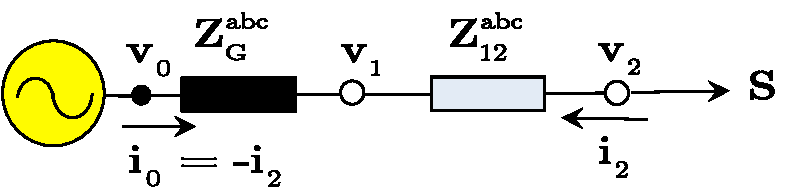
\includegraphics[width=4in]{images/pf2.pdf}
  \caption{Three-phase power flow}\label{fig:5}}
\end{figure}
\newpage

Let us define $a$=$e^{\frac{2 \pi i}{3}}$, starting with $\bm{v_2}$=$\bm{v_0}$=$\frac{12.47}{\sqrt{3}}[1, a^2, a]^T$, using KVL we update $\bm{v^{new}_2}$ as

\begin{equation}
  \bm{v^{new}_2}=\bm{v_0}+(\mathbf{{Z}^{abc}_{G}}+\mathbf{{Z}^{abc}_{12}})\cdot \bm{i_2}\mbox{ kV}
\end{equation}


where $\bm{i_2}=[i^a_2, i^b_2,i^c_2]T=conj([\frac{-{S^a}}{{v}^a_2},\frac{-{S^b}}{{v}^b_2},\frac{-{S^c}}{{v}^c_2}]^T)$

After a number of iterations (\textit{iter}) when $\mid{v}^{p,new}_2-{v}^{p, old}_2\mid\leq \epsilon$ for all phase $p$=$a,b,c$, the loop stops. Thus, voltage at bus 1 is:

\begin{equation}
  \bm{v_1}=\bm{v_0}+\mathbf{{Z}^{abc}_{G}}\cdot \bm{i_2}\mbox{ kV}
\end{equation}

In matricidal form, resulting voltages and currents are:

\begin{equation}
  \bm{v}=[\bm{v_0}, \bm{v_1},\bm{v_2}]^T
\end{equation}
\begin{equation}
  \bm{i}=[-\bm{i_2},[0;0;0],\bm{i_2}]^T
\end{equation}

Applying the Tellegen's theorem, power losses at the line are: $\Delta {S}$=$\Delta P$+j$\Delta Q$ 
=$3*[\bm{v_1},\bm{v_2}][-\bm{i^*_2},\bm{i^*_2}]^T$

\subsection{Power Flow No. 6: Newton Method (Three-phase)}

Given the three-phase nominal voltage ($v_0=12.47/\sqrt{3}$), the source Th\'evenin equivalent impedance matrix ($\mathbf{{Z}^{abc}_{G}}$), the network series impedance ($\mathbf{{Z}^{abc}_{12}}$), shunt admittance ($\mathbf{{Y}^{sh,abc}_{12}}$) and total load ($\bm{S}$),
determine voltages ($\bm{v}$), injected currents ($\mathbf{i}$), active power (losses) and computational performance:
    
\begin{verbatim}
[V,I,losses]=Newton_3(zgabc,zabc,Sabc,yshabc);% Newton method
\end{verbatim}

The idea is find $\bm{v}$=$[\bm{v_1},\bm{v_2}]^T$ from $\bm{i}$=$\mathbf{Y^{abc}_{BUS}}\bm{v}$ (Eq. \ref{4}) using an appropriate solver (Octave's {fsolve} tool).


\begin{equation}
 \left[ \begin{array}{ccc}\label{4}
 \mathbf{{Y}^{abc}_{G}} & - \mathbf{{Y}^{abc}_{G}}  &\mathbf{0} \\
 - \mathbf{{Y}^{abc}_{G}} &  \mathbf{{Y}^{abc}_{G}+{Y}^{abc}_{12}+\frac{1}{2}{Y}^{sh,+}_{12}} & -\mathbf{{Y}^{abc}}_{12}\\
 \mathbf{0} & -\mathbf{{Y}^{abc}_{12}} & \mathbf{{Y}^{abc}_{12}+\frac{1}{2}{Y}^{sh,+}_{12}}
             \end{array}
           \right]
  \begin{bmatrix}
  \bm{v_0}\\ 
	\bm{v_1}\\ 
	\bm{v_2}
\end{bmatrix}
  =
  \begin{bmatrix}
\bm{i_0}=-\bm{i_2}\\ 
\bm{0}\\ 
\bm{i_2}
\end{bmatrix}
  \end{equation}
where $\bm{i_2}=[i^a_2, i^b_2,i^c_2]^T=conj([\frac{-{S^a}}{{v}^a_2},\frac{-{S^b}}{{v}^b_2},\frac{-{S^c}}{{v}^c_2}]^T)$. Applying the Tellegen's theorem, power losses at the line are: $\Delta {S}$=$\Delta P$+j$\Delta Q$ 
=$3*[\bm{v_1},\bm{v_2}][-\bm{i^*_2},\bm{i^*_2}]^T$


%Following the notations set down in \cite{Cur_Zw}, we consider   retarded delay differential systems
% in the form
%\begin{align}
%\dot{x}(t)&= A_0x(t) +\sum_{j=1}^p A_j x(t-h_j) +B_0u(t) +D_0(t), \label{delay_eq1}\\
%x(0)&=r \in   \bbr^n,  \label{delay_eq2}\\
%x(\ta)&=\vp \in L^2([-h_p,0],\bbr^n) \label{delay_eq3}\\
%&0< h_1< \cdots <h_p ,\ \ \text{are delays}\nonumber\\
%y(t)&=C_0x (t). \label{delay_eq4}
%\end{align}
% As in \cite{Cur_Zw} we
%denote  by  $x(t)\in
%\bbr^n$ the state of the system,
%$A_j\includegraphics{
%\call (\bbr^n)$, for
%$j=1,
%\cdots ,p$. The input operator  is given by
%$B_0\in \call(\bbc^m,\bbc^n)$ for inputs  $u\in L^2([0,\tau],\bbc^m)$ for all $\tau>0$, and the output
%operator $C_0\in
%\call(\bbc^n,\bbc^m)$. It can be shown  (see for example
%\cite{Cur_Zw}) that the solution to
%\eref{delay_eq1}-\eref{delay_eq3} with $u=0$ and $D_0=0$ can be expressed as
%\begin{equation}\label{delay_eq5}
%x(t)=e^{A_0 t} r + \sum_{j=1}^p \int_0^t e^{A_0(t-s)} A_jx(s-h_j)\, ds.
%\end{equation}
%
%We can also formulate this problem in a standard state space format in the infinite
%dimensional state space (cf, \cite{htb1},  \cite{htb3}, \cite{Cur_Zw})
%\begin{equation}\label{delay_eq6}
%\sZ=\bbc^n\oplus L^2([-h_p,0],\bbc^n),
%\end{equation}
%with inner product in $\sZ$ is given by
%\begin{equation}\label{delay_eq7}
%\left \lag Z_1,Z_2
%\right\rag =\lag r_1,r_2\rag_{\bbc^n} +
%\lag \vp_1,\vp_2\rag_{L^2}, \ \ \ Z_1=\begin{pmatrix}r_1\\\vp_1(\cdot)\end{pmatrix},\ \
%Z_2=\begin{pmatrix}r_2\\\vp_2(\cdot)\end{pmatrix}.
%\end{equation}

\begin{thebibliography}{100}

%\bibitem{2} Sunderman, W. G., Dugan, R., Dorr, D. S. (208). The neutral-to-earth voltage (NEV) test case and distribution system analysis. 
\bibitem{1} W.H. Kersting, "A three-phase unbalanced line model with grounded neutrals through a resistance,"  \textit{In Proc.  IEEE PESGM'08}, 208, pp.  1-7.
\bibitem{2} Kersting, W. H. (2018). Distribution System Modeling and Analysis. CRC Press.
\end{thebibliography}




\end{document} 